\documentclass[tikz]{standalone}
\usetikzlibrary{calc}
\usetikzlibrary{decorations,positioning}
\usetikzlibrary{decorations.markings}

\begin{document}
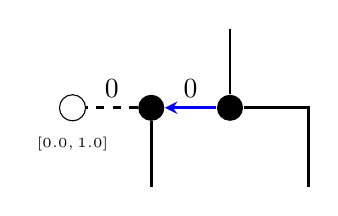
\begin{tikzpicture}[node distance=2.5cm]
	\node[circle, fill=black] (contact_source) at (0,-1) {};
	\node[circle, fill=black] (contact_destination) at (-1,-1) {};
	\node[circle, draw=black, fill=white, label={[yshift=-24pt]\tiny$[0.0, 1.0]$}] (contact_destination_filter) at (-2,-1) {};
	\draw[line width=1pt] (0,0) edge (contact_source);
	\draw[->, >=stealth, blue, line width=1pt] (contact_source) -> (contact_destination) node [midway, yshift=0.25cm, black] {$0$};;
	\draw [decorate, dashed, line width=1pt] (contact_destination) -- (contact_destination_filter) node [midway, yshift=0.25cm] {$0$};
	\draw[line width=1pt] (contact_destination) -- (-1, -2);
	\draw[line width=1pt] (contact_source) -| (1, -2);
\end{tikzpicture}
\end{document}